\section*{Introduction}
  \phantomsection
  Informational technologies play a leading role in people lives today. Robotics, as a branch of IT, is becoming more and more promising for a wide range of tasks. It deals with the design, construction, operation, and application of robots, as well as computer systems for their control, sensory feedback, and information processing, \cite{robotics}. The main advantage robots have over an ordinary computer is their mobility and possibility to move. The wide range of input and output devices incorporated into them make it possible for robots to accomplish things which only a human could do a few decades ago. The complexity of the jobs they do is achieved through data processing and Artificial Intelligence (AI). One of the most successful branches of AI is Machine Learning. Machine Learning is ``the field of study that gives computers the ability to learn without being explicitly programmed'', \cite{tooBigToIgnore}. This is the key to make sense out of the big amount of input data a robot has. Sounds, images, tactile data are translated into speech, vision and touch events. 

  The scope of this thesis is to analyze and design an object clustering system for NAO robot. Given a set of random objects which the robot can move, the system should detect the objects using Computer Vision, detect patterns and group these objects using Machine Learning then perform the movement of these objects to the corresponding group using robot's functionality. The given task is solved using image processing, clustering algorithms and robot's capabilities of locomotion. In this scope, clustering is taking one set of objects which are mixed and returning multiple sets each with identical or similar objects. Clustering is sorting, grouping of objects. This thesis is also concerned about human-robotic interaction. It also presents a way how to determine the distance to an object from the image. 

The combination of Machine Learning and Robotics is a very popular trend in today's research. A significant obstacle towards the benefits which a smart robot would provide remains the lack of needed processing power and the complexity of the tasks to process. One of such tasks is the interpretation of images acquired by camera -- a field called Computer Vision. 

  A particular example of robots is the humanoid NAO, presented in figure \ref{naoRobot}. In 2008 Aldebaran Robotics publicly released their first version of NAO robot -- an autonomous, programmable humanoid. Right from the start, NAO replaced Sony's robot Aibo in the RoboCup competition. The simplicity of usage, well-documented SDK available in 8 programming languages makes NAO an attractive platform for researchers and in academia. Since then, NAO robot became a de facto standard in robotics research, used in dozens of universities around the world, \cite{naoWiki}. In June 2014, Aldebaran released the next generation humanoid: Pepper. It contained some improvements compared to NAO.

NAO provides the platform. It is a machine, which can move (walk), has loudspeakers, microphones, video cameras, tactile sensors and an onboard computer. It has dozens of mechanical joints and on each of them a small motor which can be powered on. NAO can recognize voice in 2 predefined languages (19 available) and can speak as well (text-to-speech functionality). The problem is that NAO is a computer which can move, but cannot think or decide by himself. He has many inputs and outputs and programmers' task is to make use of them. He has two cameras, but he cannot detect objects. He has hands, but there is no such functionality as ``grab that object''. In this context Machine Learning can make sense out of the big amount of input data that NAO has.

  This thesis is composed of five chapters. The first chapter is dedicated to detailed problem description and analysis of the domain. In this chapter similar works, the used technologies, frameworks and the robot itself are described. The second chapter provides an explanation of the algorithms used in this project. Image processing algorithms, clustering methods and distance calculation are presented from mathematical point of view. The third chapter is concerned with the modeling of the software. The system is designed through UML diagrams and the used API-s are described. The workflow and the process of the implementation is described in detail. Different issues and the way they where tackled are presented. Finally the forth chapter presents an economical insight into the project, what are the costs and how the assets loose their value due to wear. The thesis ends with the conclusion, UML diagrams and the source code of the program. 

\begin{figure}[!ht]
\renewcommand\thefigure{I.1} % Make this Figure I.1
\centering
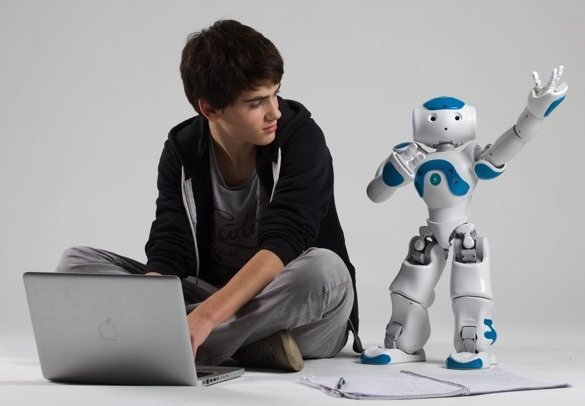
\includegraphics[width=15cm]{1.png}
\caption{Fully programmable NAO humanoid robot, \cite{naoPhoto1}}\label{naoRobot}
\end{figure}

\clearpage